\begin{figure}[H]
  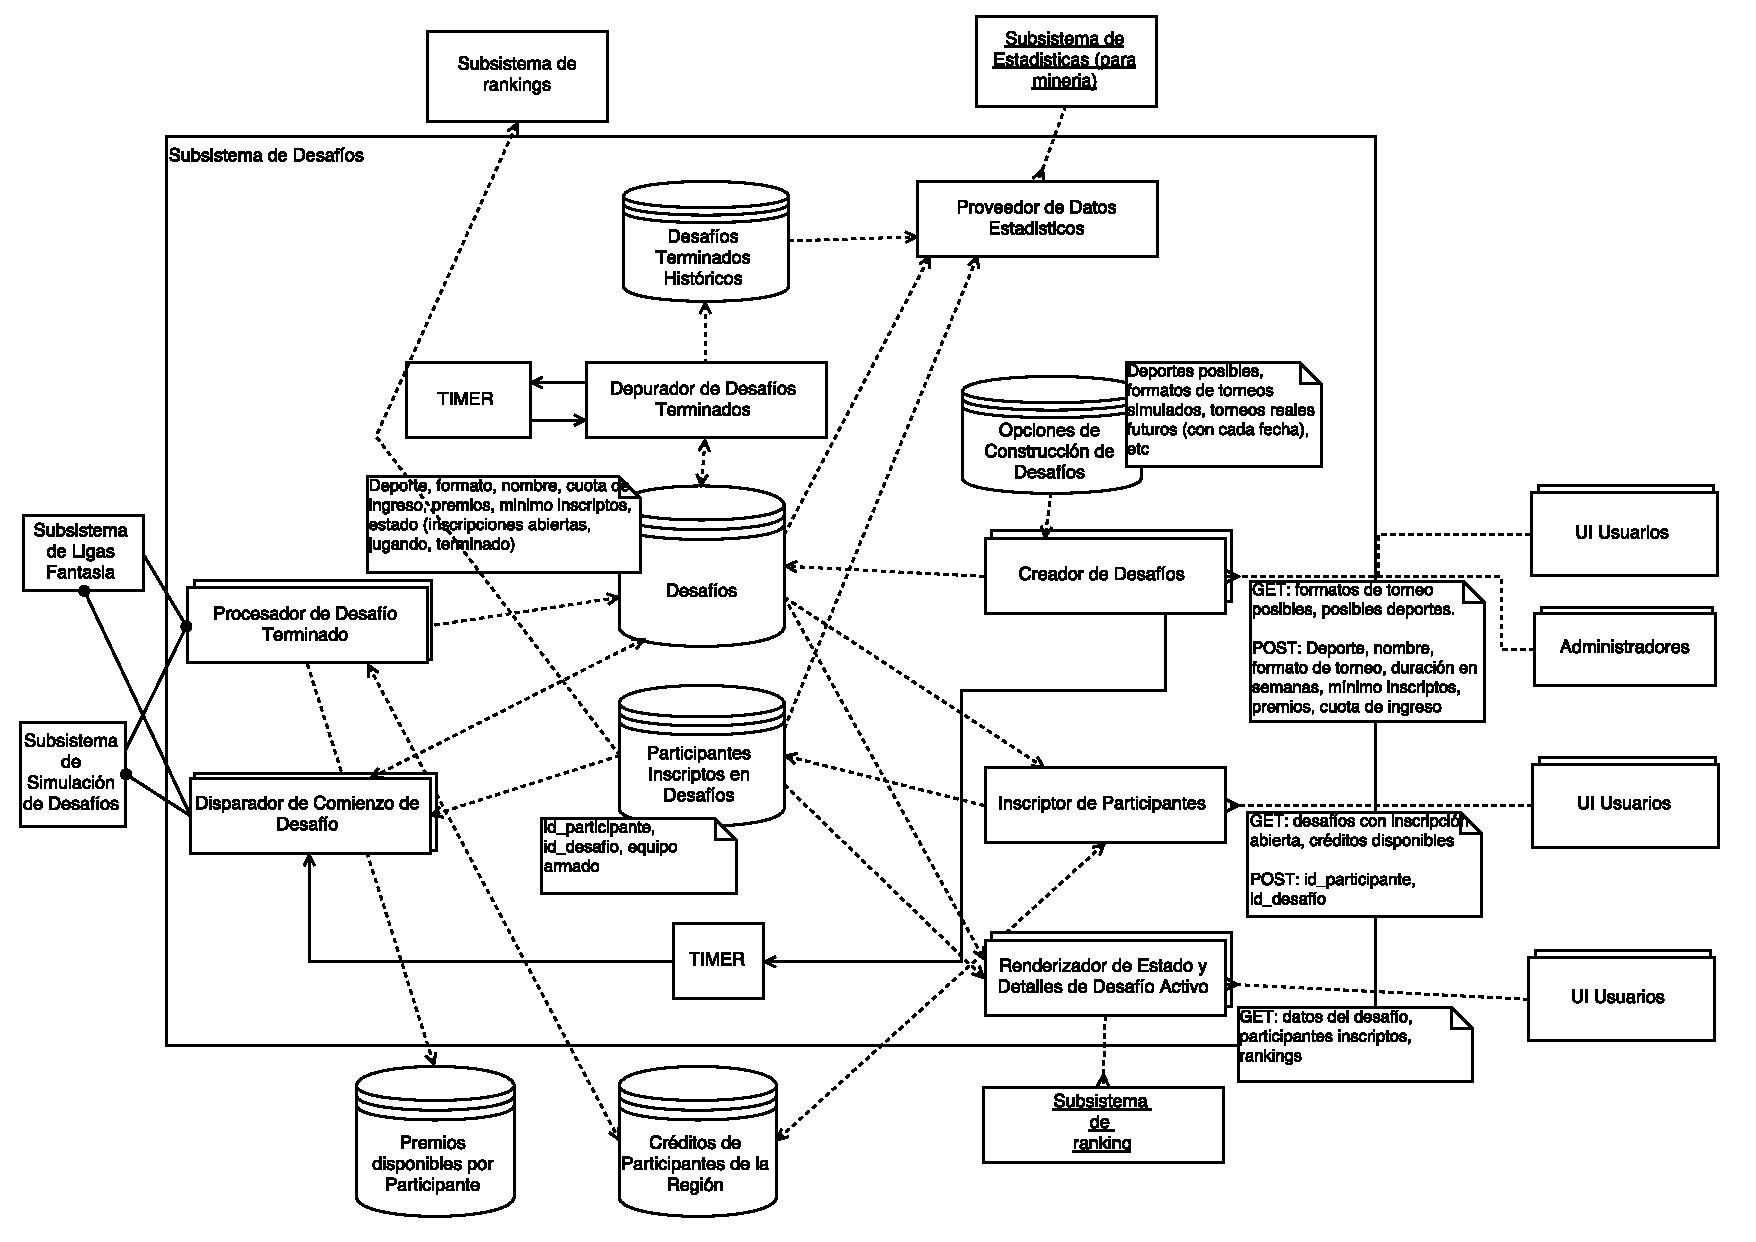
\includegraphics[width=1.1\textwidth, page=1, clip, trim=10 0 10 0]{imagenes/Subs-desafios.pdf}
  \caption{Subsistema de Desafios.}
\end{figure}
% \newpage
El subsistema de desafíos se encarga de crear desafíos, inscribir participantes, iniciar desafios en el momento indicado, proveer detalles y estado de cada desafio a los usuarios.
Cuando un desaífo comienza se encarga de informar al subsistema de simulación o liga de fantasia seúgn corresponda. Además se encarga de cobrar créditos de inscripción y de pagar premios (tanto en créditos como premios especiales, que luego los usuarios podrán cambiar por el premio real en dinero o lo que corresponda. También provee una interfaz de consulta de estadísticas de desafios.\\

\begin{itemize}
\item Desafíos Terminados: Los desafíos finalizados durante la última semana van a tener más solicitudes de consulta de estado. Es por esto que esos desafíos se mantienen
en el repositorio principal de desafíos con redundancia activa para mejorar la disponibilidad y la performance. Pasados los 7 días de finalizado, un proceso que ejecuta una vez por día se encarga de depurar el repositorio principal para mejorar la performance de las búsquedas, asumiendo que esos desafíos serán consultados con menos frecuencia.

\item Creador de Desafíos: Devuelve todas las opciones posibles para construir un desafío (tanto para modo simulado como para modo liga de fantasía). Luego recibe la configuración elegida y crea el desafío. Se almacena en un repositorio local que luego se propaga a todas las réplicas regionales.

\item Inscripción de participantes: Muestra una lista con todos los desafíos por cada deporte (tanto simulados como liga de fantsía) que aún estén con la inscripcion abierta (aún no comenzaron ajugarse). Por cada uno muestra el valor en creditos para ingresar. Luego se inscribe un participante (siempre y cuando ls créditos le alcancen). Para mejorar la performance y disponibilidad (muchos podíran intentar inscribirse a la vez), luego de hacer el checkeo se guardan en una caché todos los pedidos de  inscripcion que luego se van persistiendo por procesos dedicados.

\item Renderizador de estado y detalles: Devuelve el estado de un desafio especifico (si está abierto a inscripciones, si se esta jugando o si está terminado) asi como también la cuenta regresiva para que empiece el desafio (y se cierren inscripciones) y todos los detalles asociados (premios, cuota de inscripción, tipo de desafío, formato de torneo o fechas que se juegan, etc.), y el ranking, si corresponde. Internamente se utiliza una caché. Cada pedido que llega se guarda en un repositorio y se solicitan los datos a un manager de cache (que se crea en el momento que se necesita) y a un proceso que busca los datos en los repositorios persistentes (tambéin se crea cuando se necesita). Si el dato llega de la caché, se mata al proceso que  fue a disco (y tambien se mata al proceso de la caché). En cambio si no estaba en la caché, el dato llegaár del disco (y ahí tambéin se guarda en la caché para soportar eficentemente un período corto de muchos pedidos de detales del mismo desafio. Un proceso se ejecuta cada 1 minuto y borra los datos de caché que tengan más de un minuto de antigüedad. Dado que los datos no deben mostrarse en tiempo real, este mcanismo mejora la disponibildad y la performance de respuesta a muchas solicitudes de detalles de un desafío popular.
\end{itemize}

\begin{figure}[H]
  \includegraphics[width=\textwidth, page=3, clip, trim=20 0 20 30]{imagenes/Subs-desafios.pdf}
  \caption{Zoom en Procesador Desafio Terminado y Creador de Desafios}
\end{figure}

\begin{figure}[H]
  \includegraphics[width=\textwidth, page=4, clip, trim=20 0 20 0]{imagenes/Subs-desafios.pdf}
  \caption{Zoom en Inscriptor de Participantes y Renderizador de Estados y Detalles Desafio Activo}
\end{figure}
